\begin{figure}[ht!]
  \centering
  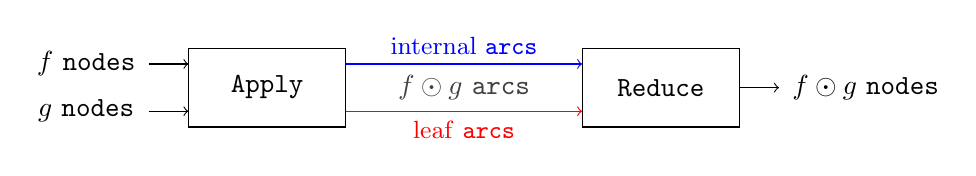
\begin{tikzpicture}[every text node part/.style={align=center}]
    % Boxes
    \draw (0,0) rectangle ++(2,1) node[pos=.5]{\texttt{Apply}}; \draw (5,0)
    rectangle ++(2,1) node[pos=.5]{\texttt{Reduce}};

    % Arcs
    \draw[->] (-0.5,0.8) -- ++(0.5,0) node[pos=-1.6]{$f$ \texttt{nodes}};
    \draw[->] (-0.5,0.2) -- ++(0.5,0) node[pos=-1.6]{$g$ \texttt{nodes}};

    \draw[blue, ->] (2,0.8) -- ++(3,0) node[pos=0.5,above]{\small\color{blue}
      internal \texttt{arcs}};

    \node at (3.5,0.5) {\textcolor{darkgray}{$f \odot g$ \texttt{arcs}}};
  
    \draw[red, ->] (2,0.2) -- ++(3,0) node[pos=0.5,below]{\small\color{red} leaf
      \texttt{arcs}};

    \draw[->] (7,0.5) -- ++(0.5,0) node[pos=3.2]{$f \odot g$ \texttt{nodes}};
  \end{tikzpicture}
\end{figure}